\documentclass[10pt, titlepage, oneside, a4paper]{article}
%\usepackage[swedish]{babel}
\usepackage[T1]{fontenc}
\usepackage[titletoc]{appendix}
\usepackage[utf8]{inputenc}
\usepackage{amssymb, graphicx, fancyhdr}
\usepackage{amsmath}
\usepackage{amsthm,algorithm,algorithmic,yhmath,enumitem,lscape}
\usepackage{float}
\usepackage{hyperref, url}
\addtolength{\textheight}{20mm}
\addtolength{\voffset}{-5mm}
\renewcommand{\sectionmark}[1]{\markleft{#1}}

\def\inst{Instutition}
\def\typeofdoc{Project}
\def\course{coursename}
\def\pretitle{Pretitle}
\def\title{Title}
\def\name{Name}
\def\username{username}
\def\email{\musername{}@cs.umu.se}
\def\path{path}
\def\graders{Graders}

\def\mfullpath{\raisebox{1pt}{$\scriptstyle \sim$}\musername/\path}
\def\nfullpath{\raisebox{1pt}{$\scriptstyle \sim$}\nusername/\path}

\newcommand{\R}{\mathbb{R}}
\newcommand{\N}{\mathbb{N}}
\newcommand{\Rn}{\mathbb{R}^n}
\newcommand{\Rnn}{\mathbb{R}^{n \times n}}
\newcommand{\bes}{\begin{equation*}}
\newcommand{\ees}{\end{equation*}}
\newcommand{\be}{\begin{equation}}
\newcommand{\ee}{\end{equation}}
\newcommand{\bms}{\begin{multline*}}
\newcommand{\emults}{\end{multline*}}
\newcommand{\bbm}{\begin{bmatrix}}
\newcommand{\ebm}{\end{bmatrix}}
\newcommand{\eps}{\epsilon}
\newcommand{\fl}{\text{fl}}
\newcommand{\Lp}{{L^p}}
\newcommand{\Ker}{\text{Ker}\,}
\newcommand{\loc}{{\text{loc}}}
\newcommand{\ccinf}{C_c^\infty}
\newcommand{\supp}{\text{supp}}
\newcommand{\dist}{\text{dist}}




\begin{document}
	\begin{titlepage}
		\thispagestyle{empty}
		\begin{large}
			\begin{tabular}{@{}p{\textwidth}@{}}
				\textbf{Gisma University \hfill \today} \\
				\textbf{Github portfolio} \\
				\textbf{Report} \\
			\end{tabular}
		\end{large}
		\vspace{25mm}
		\begin{center}
			\LARGE{\pretitle} \\
			\huge{\textbf{Computer Science Portfolio }}\\
			\vspace{10mm}
			\LARGE{\title} \\
			\vspace{15mm}
            \LARGE{GOOGLE CYBER SECURITY} \\
            \vspace{10mm}
			\begin{large}
				\begin{tabular}{ll}
					\textbf{Name} & Alvan Sameri \\
					\textbf{Student Number} & GH1058624
				\end{tabular}
			\end{large}
			\vfill
            \vfill
			\large{\textbf{Graders}}\\
			\mbox{\large{\graders}}
		\end{center}
	\end{titlepage}
    
    % fixar sidfot
	\lfoot{\footnotesize{\name, \username}}
	\rfoot{\footnotesize{\today}}
	\lhead{\sc\footnotesize\title}
	\rhead{\nouppercase{\sc\footnotesize\leftmark}}
	\pagestyle{fancy}
	\renewcommand{\headrulewidth}{0.2pt}
	\renewcommand{\footrulewidth}{0.2pt}

	% skapar innehållsförteckning.
	% Tänk på att köra latex 2ggr för att uppdatera allt
	\pagenumbering{roman}
	\tableofcontents
	% och lägger in en sidbrytning
	\newpage

	\pagenumbering{arabic}

	% i Sverige har vi normalt inget indrag vid nytt stycke
	\setlength{\parindent}{0pt}
	% men däremot lite mellanrum
	\setlength{\parskip}{10pt}

\section{Abstract}
This is a report presenting the design, implementation, and content of my Computer Science Portfolio.As the Portfolio was developed to show case evidence of skills and projects that I have worked on. It show case links to github that houses the project. The project available on github include a live link to a working portfolio website\url{https://alvansameri-collab.github.io/myproject/}.It also contain a cv \url{https://github.com/alvansameri-collab/alvan-sameri-cv}and also a general report to all the project \\



This report shows and discusses the objectives of the project ,the structure of the website, the github repository, the technologies and the tools used during this development. Furthermore, the report shows an evaluation of the final product, examines the strengths and limitation of the portfolio and identifies opportunities for future improvement. It tries also to demonstrate practical application of webdevelopment and the importance of maintaining a professional digital presence within the field of computer studies \\



\section{Introduction}
Today's world having an online portfolio where you can display your work and skills is important.Espesially in this rapid  digital technology growth. As a result more campanys have used this to identify students, graduates and professinals who are skilled and have showcase their work and projects as prof of this skills. This elliminates traditional paper written resumes as unlike trditional one it provides a dynamic and interactive platform though which you can show case academic achievements and professional experiences. It is proven that in this modern age, employers greatly increase their rely on online resources while evaluating the potential of a candidate for internships, employment opportunities and professional collaboration. \\



Creating of a personal portfolio website has been one of the most effective methods of establishing. A portfolio website serves as a digital representation of an individual's skills, projects, experiences and achivements unlike traditional curriculum vitae documents, portfolio website allows visitors to interact with content in the right engaging manner while providing access to examples of practical work and technical accomplishment \\


This was a project in which its purpose was designing and developing a computer science portfolio website capable of presenting information in a clear, organized and professional format.The website was developed using HTML and included image that enhance the visual presentation of the project\\
In addition to the website development, the project involved the creation of a github repository to store my personal cv and the project report\\
This report provides a comprehensive overview of the portfolio development process. It examines project objectives, design considerations, implementation procedures, testing activities, strengths, weaknesses, and future enhancements. Through this analysis, the report demonstrates how the project successfully fulfilled its intended purpose while contributing to the development of practical technical skills\\
The website is hosted through GitHub Pages and is publicly accessible.This report examines the complete project, including website content, repository structure, technical artifacts, design considerations and future development opportunities.

Report \url{https://github.com/alvansameri-collab/Project-report} \\
Curriculam vitael \url{https://github.com/alvansameri-collab/alvan-sameri-cv} \\
Porlfolio website \url{https://alvansameri-collab.github.io/myproject/} \\
Github \url{https://github.com/alvansameri-collab/}

\section{Project Objectives}

The project primary objective was to develop a professional portfolio website capable of presenting information in a clear and accessible format. It also tries to include a Github repository which it content include a personal cv and a portfolio website. Specific goals were creating a functional HTML based website, providing a curriculum vitae and uploading it to Github,helping with project presentation.



\section{Portfolio Website}

\begin{figure}[H]
    \centering
    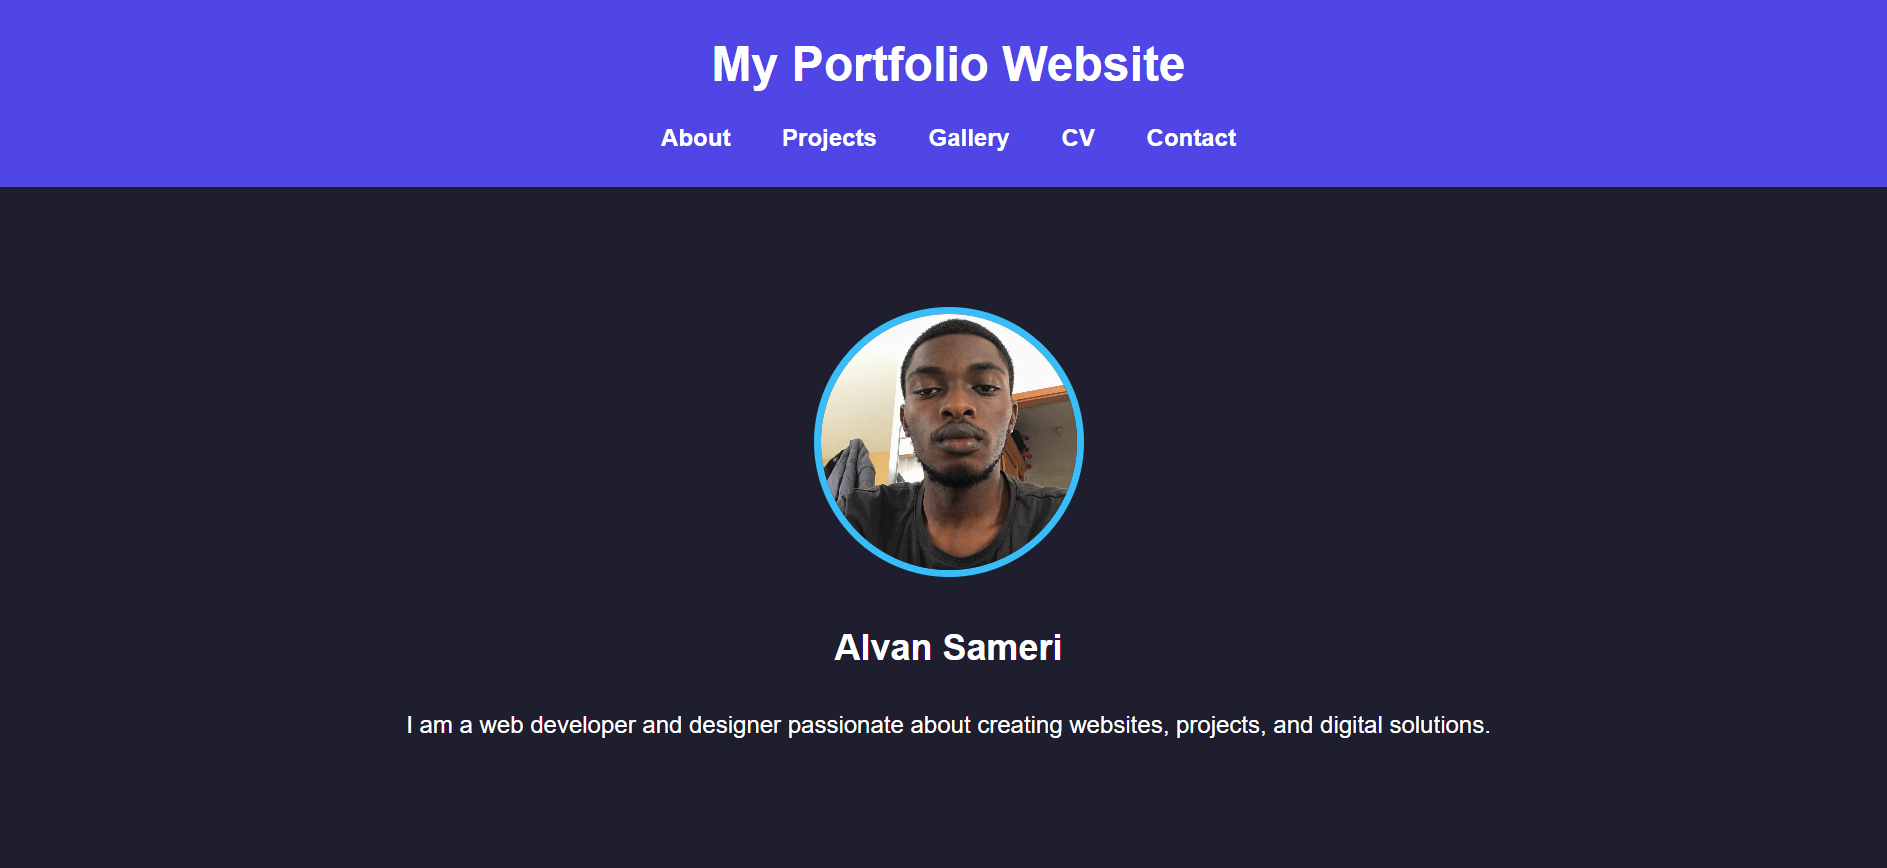
\includegraphics[width=0.9\textwidth]{portfolio.png}
    \caption{Homepage of the Portfolio Website}
    \label{fig:portfolio}
\end{figure}

\url{https://alvansameri-collab.github.io/myproject/} \\

The portfolio website is designed to be simple and easy to navigate, as it introduce its visitors to the owner. It showcases profile image ,contact information ,images of project and personal Cv \\ 

The website also gives more relevant information. The website is intended for various users including employers recruiters, lecturers, fellow students and professionals. Thus giving out qualification and technical skills to the intended audience. Unlike printed documents the portfolio website can be updated overtime whenever new projects or skills are acquired


\section{Github Repository}

\begin{figure}[H]
    \centering
    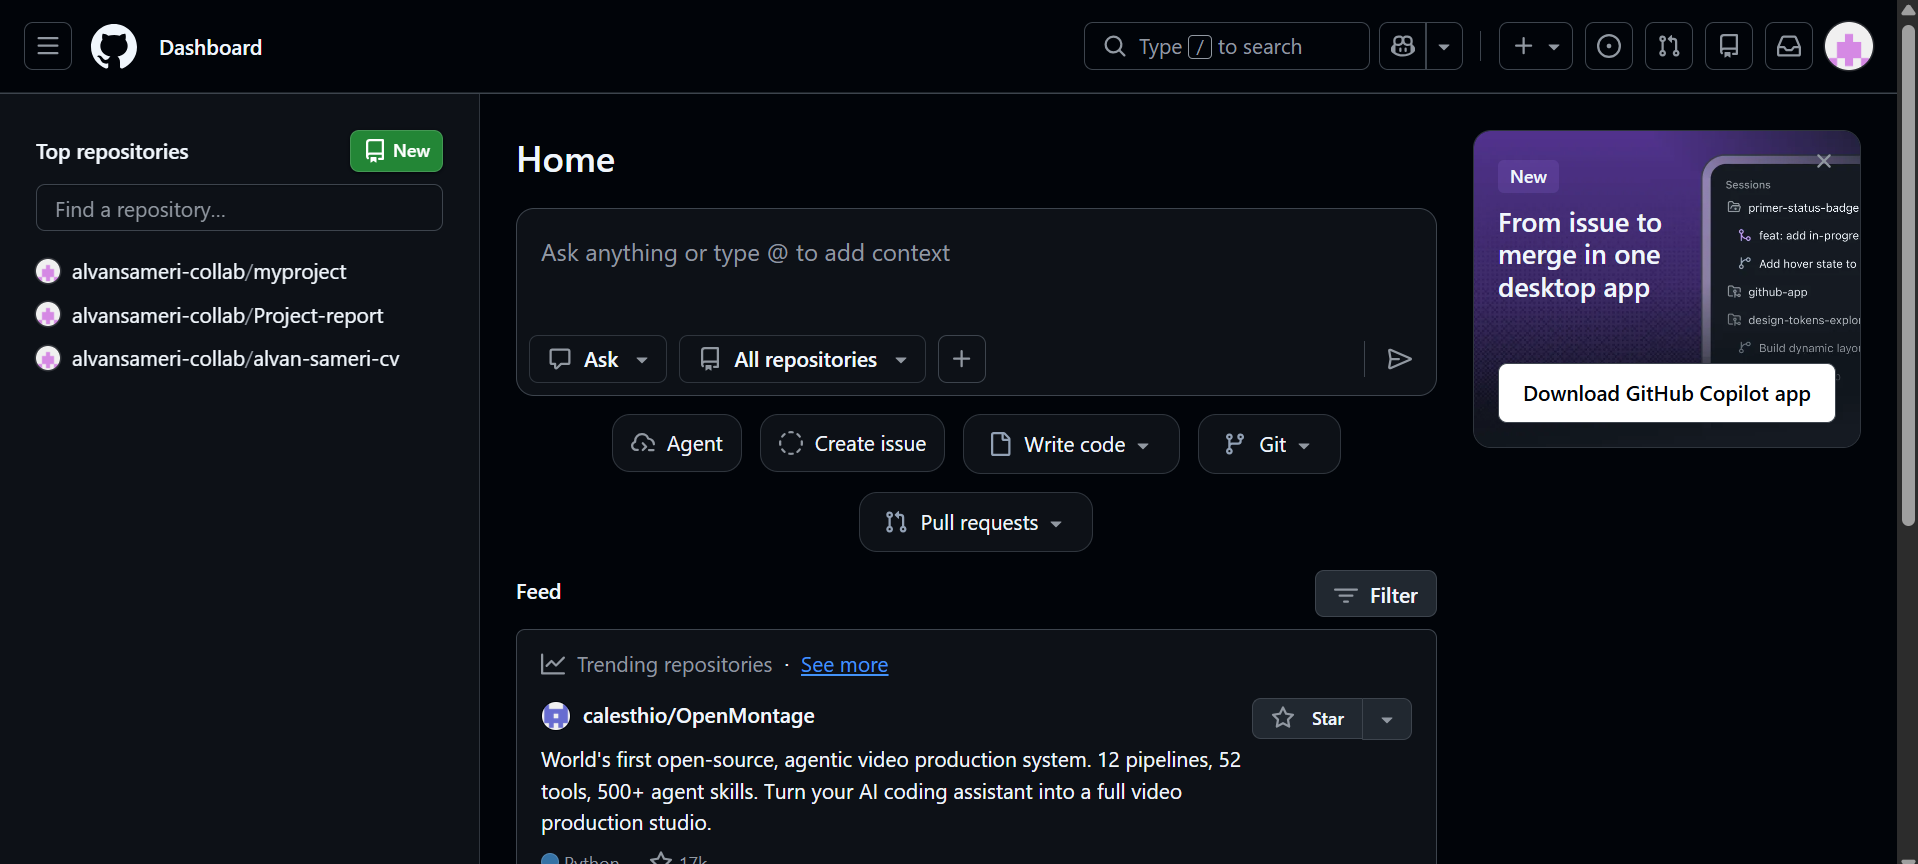
\includegraphics[width=0.9\textwidth]{github-repository.png}
    \caption{GitHub Repository Containing Portfolio Files}
    \label{fig:githubrepo}
\end{figure}

\url{https://github.com/alvansameri-collab/} \\

The Github repository is the most important part of the project...

The Github repository is the most important part of the project. As it houses all the required files for the website. The files include item.html and images. Github also contain a personal curriculum vitae. \\
It also provides live links to an active portfolio website that is stored in there.Te projects are public and available for anyone to view and provide comments on it.

\section{Curriculum Vitae}

\begin{figure}[H]
    \centering
    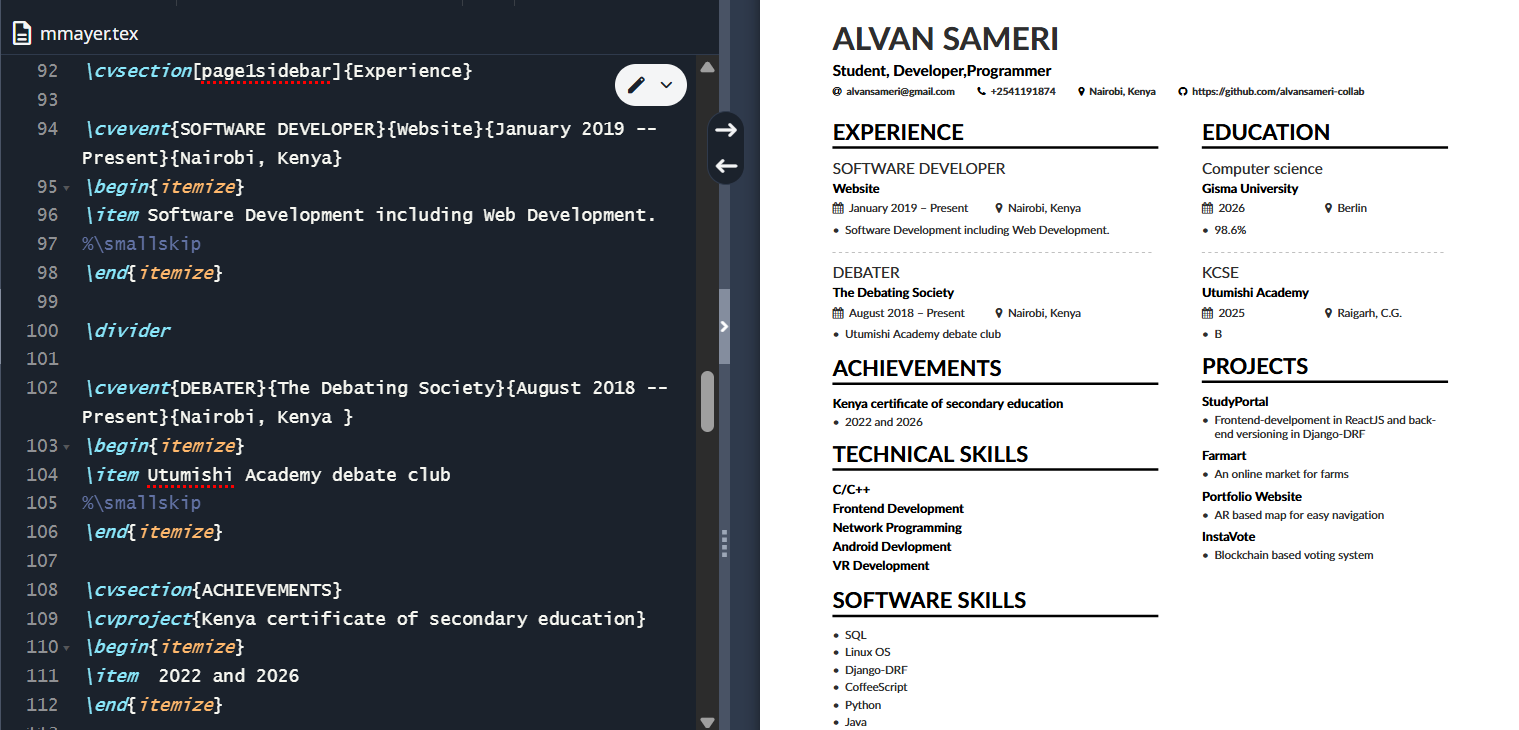
\includegraphics[width=0.8\textwidth]{cv-screenshot.png}
    \caption{Curriculum Vitae Available Through GitHub Repository}
    \label{fig:cv}
\end{figure}

\url{https://github.com/alvansameri-collab/alvan-sameri-cv} \\
The Curriculum vitae is an important document the visitors can access a formal summary of qualifications, educational background, technical competencies and professional achievements. Including the curriculum vitae into the repository increase the usefulness of the portfolio and provide recruiters with additional information. \\

 \section{Strengths and Weaknesses}
 The project show case several strengths and weakness \\

 On the strengths the portfolio is simple,easy to navigate and public accessible. One can access the portfolio website and the curriculum vitae. The use of Github Pages provides  reliable hosting, while the repository structure remains easy to understand and maintain. \\

 Another strength is the use of GitHub as a development platform. The repository demonstrates familiarity with version control concepts and provides transparency regarding project organization. \\

 Despite these strengths, the project has limitations. The website is primarily static and does not include advanced interactive features. Content updates require manual editing of source files. There is currently no database integration or backend functionality.

Despite this limitations, it still does not prevent the portfolio from achieving its objectives and it opens windows for future advancement.

\section{Technologies and Tools Used}

HTML as the most important tool. It provided the structural framework required for website development and enable the presentation of text, images and links \\

GitHub played an important role as it was used for both repository hosting platform and a deployment solution of the website.As through Github pages the website could be published without requiring separate hosting app. \\

Git was used as a tool to enable projects changes over time. This is important for software development by providing accountability and support future maintenance. \\

Latex was also involved as a language tool to write both the cv and the report. This language enabled visual presentation of this documents in both visual and coded form \\
 

\section{Future improvement}

There is chances of future development to enable the portfolio to expand its capabilities significantly.Also adding additional styling to improve usage experience. \\
Alive video link could be added that gives more visual experience \\ 
A chat box could be added to allow the public to give their feedback on the portolio website 
\\
JavaScript functionality could also be added to introduce interactive features such as animation.The repository could also be expanded to include additional projects, technical documentation and coding samples. \\
The personal curriculum vitae can also be improved by updating the experience and education background.

\section{Conclusion}

The portfolio website and GitHub repository has achieved its objective by providing a professional platform for presenting your information and technical skills.Through tools like HTML, GitHub and GitHub Pages a portfolio was developed and published online \\

In general the project showed web development skills, repository presentation skills and showing professional online presentation. \\
The presents of the curriculum vitae and Images gives strength the overall portfolio making it useful for recruiters, lectures and industry professionals. \\ 
As the project displays more room for improvement, allowing one to add resent work into the portfolio

\end{document}